\section{Methodik und Projektvorgehen}
\label{sec:methodik}

Die Qualität einer wissenschaftlichen Untersuchung im Bereich Deep Learning hängt maßgeblich von der Datenbasis und den gewählten Modellarchitekturen ab. In diesem Kapitel wird das methodische Vorgehen von HSP 2 erläutert. Dies umfasst die Auswahl und Aufbereitung der Daten aus dem Road Damage Dataset 2022 (RDD2022) sowie die detaillierte Beschreibung der untersuchten Transformer-Architekturen. Zudem wird die mathematische Grundlage der Evaluationsmetriken definiert, um eine objektive Bewertung der Ergebnisse zu ermöglichen. Der Fokus liegt dabei auf einer klaren Strukturierung des Prozesses von der Datenerfassung bis zur statistischen Auswertung.

\subsection{Datenbasis: Das Road Damage Dataset 2022 (RDD2022)}
Für HSP 2 wurde das Road Damage Dataset 2022 (RDD2022) als primäre Datenquelle gewählt. Es handelt sich um eine der weltweit umfangreichsten Datenbanken für Straßenschäden, die speziell für die Forschung im Bereich Computer Vision entwickelt wurde. Der Datensatz enthält zehntausende Aufnahmen aus sechs verschiedenen Ländern: Japan, Indien, Tschechien, Norwegen, USA und China.

\paragraph{Die Bedeutung der internationalen Vielfalt}
Die Einbeziehung von Daten aus verschiedenen Ländern ist für die Robustheit der Modelle von zentraler Bedeutung. Straßenszenen unterscheiden sich international erheblich. Aus technischer Sicht dient diese Vielfalt als eine Form der \textbf{Domänen-Varianz}.
\begin{itemize}
    \item \textbf{Umweltbedingungen:} Die Lichtverhältnisse variieren von der grellen Sonne in Indien bis hin zu den oft bewölkten oder regnerischen Bedingungen in Norwegen. In der Informatik ist dies eine Herausforderung für die Helligkeits-Invarianz der Modelle.
    \item \textbf{Infrastruktur:} Die Qualität des Asphalts, die Art der Fahrbahnmarkierungen und sogar die Farbe der Gesteinskörnung im Asphaltgemisch unterscheiden sich je nach Land.
    \item \textbf{Fahrzeuge und Umgebung:} Objekte im Hintergrund, wie spezifische Fahrzeugtypen oder länderspezifische Vegetation, können Modelle ablenken, wenn diese nicht auf eine hohe Varianz trainiert werden.
\end{itemize}
Diese Vielfalt zwingt die Modelle in HSP 2, allgemeingültige Merkmale für Risse und Schlaglöcher zu lernen, anstatt sich auf spezifische Hintergründe zu spezialisieren (Vermeidung von Overfitting auf die Umgebung).

\paragraph{Vom Detektions- zum Klassifikationsdatensatz}
Ursprünglich ist das RDD2022 für die Objekterkennung (Object Detection) konzipiert. Schäden sind in den Bildern durch Rahmen (Bounding Boxes) markiert. Da das Ziel von HSP 2 jedoch die hochpräzise Klassifizierung der Schadensart ist, war eine Transformation der Daten notwendig. Mit diesem Schritt wird das ursprüngliche Detektionsproblem in ein reines Klassifikationsproblem überführt, um die Kapazität der Transformer voll auszuschöpfen.

Aus den Originalbildern wurden die annotierten Bereiche extrahiert. Ein automatisches Skript wurde entwickelt, um die oft rechteckigen Bounding Boxes symmetrisch zu quadratischen Bildkacheln (Patches) zu erweitern. Dabei wurde ein Puffer von 10\% zur Seitenlänge addiert, um den Übergang vom Schaden zum gesunden Asphalt einzubeziehen. Alle extrahierten Patches wurden anschließend auf die einheitliche Zielgröße von $224 \times 224$ Pixeln skaliert. Durch diese Fokussierung kann das Modell seine volle Kapazität auf die Analyse der Schadenscharakteristik verwenden.

\paragraph{Definition der Schadensklassen}
Der Datensatz orientiert sich an international standardisierten Schadensklassen, die auch für die deutsche Straßenzustandsbewertung (ZTV ZEB) von hoher Relevanz sind:
\begin{itemize}
    \item \textbf{D00 (Längsriss):} Diese Risse verlaufen parallel zur Fahrtrichtung. Sie entstehen oft durch Ermüdung des Asphalts in den Radspuren.
    \item \textbf{D10 (Querriss):} Diese Risse verlaufen senkrecht zur Fahrtrichtung. Sie sind meist die Folge von thermischen Spannungen bei Kälte.
    \item \textbf{D20 (Netzriss):} Ein komplexes Muster aus vielen kleinen, miteinander verbundenen Rissen (Alligator Cracking). Dies ist ein Zeichen für ein fortgeschrittenes strukturelles Versagen der Tragschichten.
    \item \textbf{D40 (Schlagloch):} Lokale Ausbrüche in der Fahrbahnoberfläche. Sie stellen das größte Sicherheitsrisiko dar.
\end{itemize}

\begin{figure}[H]
    \centering
    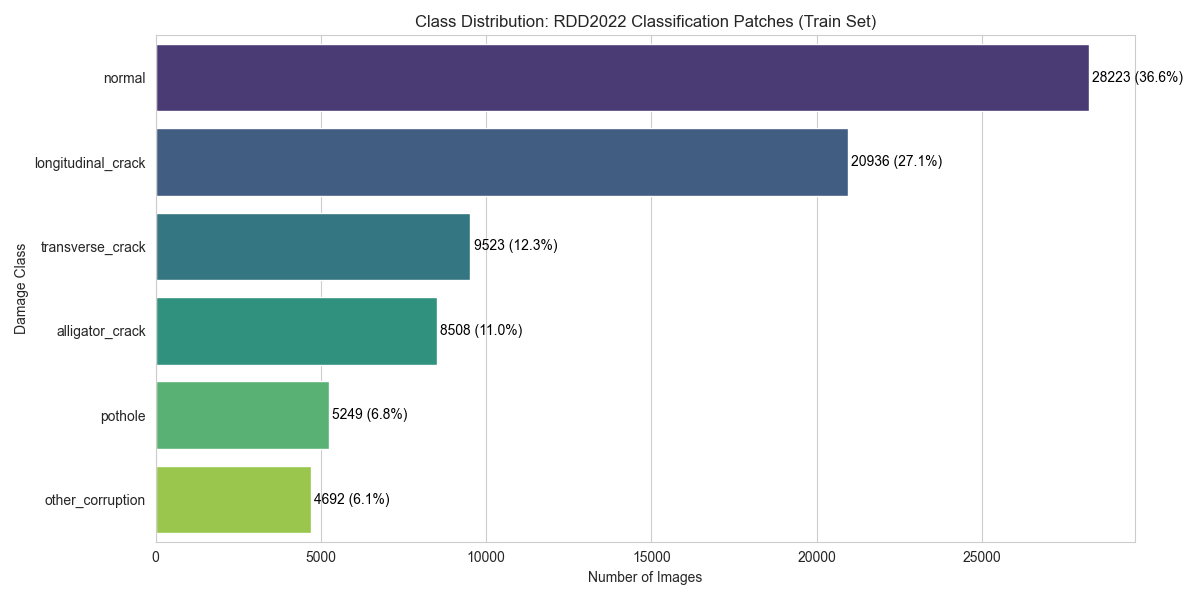
\includegraphics[width=0.75\textwidth]{../Python/hsp2_transformer/results/dataset_distribution.png}
    \caption{Statistische Verteilung der extrahierten Bildkacheln über die Schadensklassen.}
    \label{fig:dataset_dist}
\end{figure}

\subsection{Detaillierte Modellarchitekturen}
Der Kern der Untersuchung ist der Vergleich zwischen dem klassischen Vision Transformer (ViT) und dem modernen Swin Transformer. Technisch betrachtet ist dies ein Vergleich zwischen globaler und hierarchischer Informationsverarbeitung.

\paragraph{Vision Transformer (ViT-B/16)}
Der Vision Transformer (ViT) betrachtet das Bild als eine flache Sequenz von Informationen. Ein Eingabebild der Größe $224 \times 224$ Pixel wird in $14 \times 14 = 196$ Patches zerlegt.
\begin{enumerate}
    \item \textbf{Lineare Projektion:} Jeder Patch wird in einen höherdimensionalen Raum (Embedding Space) projiziert. Man kann sich das als eine Übersetzung der Pixeldaten in eine „Sprache“ vorstellen, die der Transformer versteht.
    \item \textbf{Position Embedding:} Da der Transformer keine Information über die 2D-Anordnung hat, wird jedem Vektor eine Positionsnummer hinzugefügt. Ohne dies wäre der Transformer „bildblind“ für die räumliche Anordnung (wie ein Buch, dessen Seiten beliebig vertauscht wurden).
    \item \textbf{Transformer Encoder:} Die Daten durchlaufen 12 aufeinanderfolgende Transformer-Blöcke. In jedem Block kommuniziert jeder Patch mit jedem anderen Patch (Globale Attention).
\end{enumerate}

\paragraph{Swin Transformer (Shifted Window Transformer)}
Der Swin Transformer führt eine hierarchische Verarbeitung ein, die ihn effizienter macht. Dies ist methodisch mit der \textbf{Divide-and-Conquer-Strategie} vergleichbar.
\begin{enumerate}
    \item \textbf{Patch Merging:} Ähnlich wie bei einem klassischen CNN wird das Bild in mehreren Stufen verarbeitet. Zwischen den Stufen werden benachbarte Patches zusammengefasst. Dies reduziert die Rechenlast, da die Sequenzlänge sinkt.
    \item \textbf{Shifted Windows:} Die Aufmerksamkeit wird nur innerhalb kleiner, lokaler Fenster berechnet. In aufeinanderfolgenden Schichten werden diese Fenster jedoch versetzt (Shift). Dadurch können Informationen auch über die Fenstergrenzen hinweg fließen, ohne dass eine rechenintensive globale Attention notwendig ist.
\end{enumerate}

\subsection{Evaluationsmetriken: Mathematische Grundlage}
Um die Forschungsfragen objektiv beantworten zu können, werden Metriken verwendet, die über die einfache Treffgenauigkeit (Accuracy) hinausgehen. Informatiker nutzen diese Metriken, um das Verhalten des Modells bei ungleich verteilten Daten (\textbf{Class Imbalance}) zu beurteilen.

\paragraph{Die Konfusionsmatrix als Basis}
Alle Metriken basieren auf den vier Grundwerten der Konfusionsmatrix:
\begin{itemize}
    \item \textbf{True Positives (TP):} Schaden wurde korrekt erkannt.
    \item \textbf{True Negatives (TN):} Schadenfreie Oberfläche wurde korrekt erkannt.
    \item \textbf{False Positives (FP):} Fehlalarm (Nicht-Schaden als Schaden erkannt).
    \item \textbf{False Negatives (FN):} Übersehener Schaden (Schaden nicht erkannt).
\end{itemize}

\paragraph{Definition der Metriken}
\begin{itemize}
    \item \textbf{Accuracy:} Der Anteil aller korrekten Vorhersagen.
    \begin{equation}
        \text{Accuracy} = \frac{TP + TN}{TP + TN + FP + FN}
    \end{equation}
    \item \textbf{Precision:} Misst, wie viele der gemeldeten Schäden wirklich existieren. Diese Metrik beschreibt die \textbf{Genauigkeit der positiven Vorhersagen}.
    \begin{equation}
        \text{Precision} = \frac{TP}{TP + FP}
    \end{equation}
    \item \textbf{Recall:} Gibt an, wie viel Prozent der echten Schäden gefunden wurden. Dies wird auch als \textbf{Trefferquote} bezeichnet.
    \begin{equation}
        \text{Recall} = \frac{TP}{TP + FN}
    \end{equation}
    \item \textbf{F1-Score:} Das harmonische Mittel aus Precision und Recall. Er ist besonders aussagekräftig, wenn eine Klasse (wie „Normal“) deutlich häufiger vorkommt als eine andere.
    \begin{equation}
        F1 = 2 \cdot \frac{\text{Precision} \cdot \text{Recall}}{\text{Precision} + \text{Recall}}
    \end{equation}
\end{itemize}

